\documentclass[border=3pt]{standalone}
% Shared preamble for the standalone figures.
\usepackage[T1]{fontenc}
\usepackage[scaled=0.9]{helvet}
\renewcommand{\familydefault}{\sfdefault}
\usepackage{tikz}
\usetikzlibrary{arrows.meta,positioning,calc}

\definecolor{ink}{RGB}{28,28,30}
\definecolor{rule}{RGB}{95,97,104}
\definecolor{muted}{RGB}{112,114,121}
\definecolor{accent}{RGB}{172,56,44}
\definecolor{probfill}{RGB}{250,244,235}
\definecolor{detfill}{RGB}{239,243,247}

\newcommand{\zone}[1]{{\fontsize{6.6}{8}\selectfont\bfseries #1}}
\newcommand{\sub}[1]{{\fontsize{7.2}{9}\selectfont\color{muted}#1}}
\newcommand{\mono}[1]{{\fontencoding{OT1}\fontfamily{cmtt}\selectfont #1}}

\tikzset{
  every picture/.style={font=\fontsize{8}{10}\selectfont, text=ink,
    >={Stealth[length=4.6pt,width=3.8pt]}},
  box/.style={draw=rule, line width=0.5pt, rounded corners=2pt, fill=white,
    minimum height=8mm, minimum width=16mm, inner sep=2pt, align=center},
  flow/.style={->, draw=rule, line width=0.6pt},
  hot/.style={->, draw=accent, line width=0.9pt},
  lbl/.style={font=\fontsize{7.2}{9}\selectfont, text=muted, inner sep=1.5pt},
}

\begin{document}
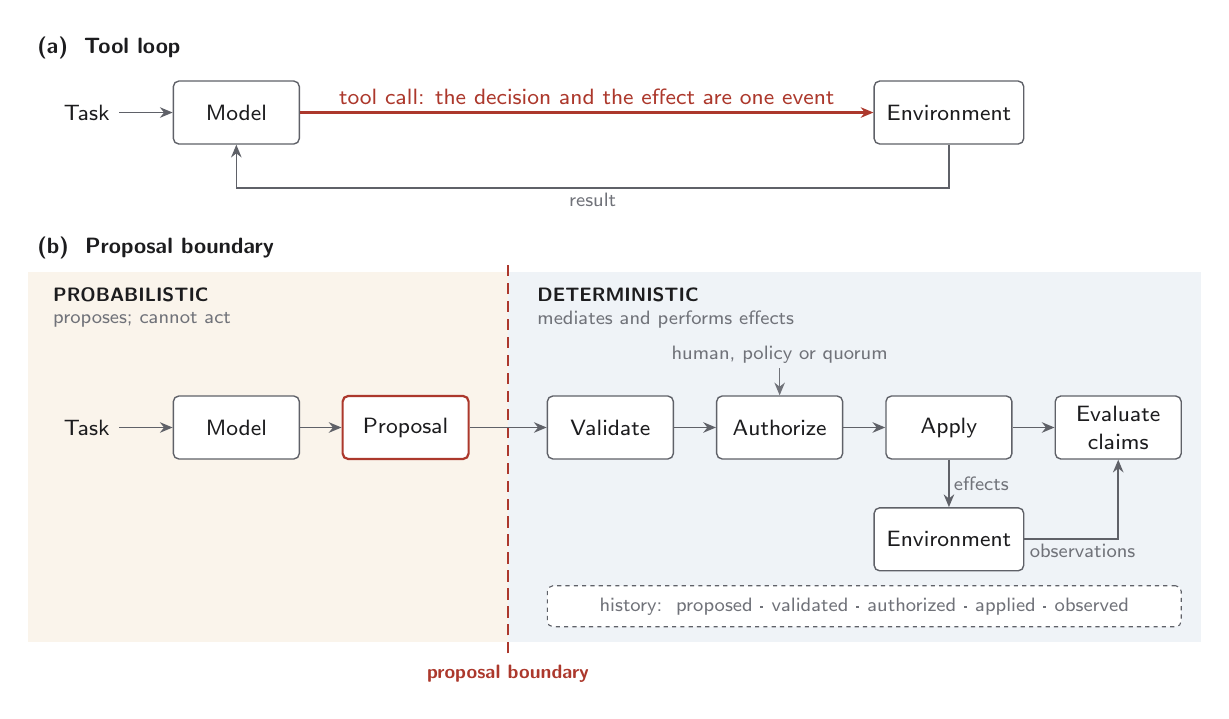
\begin{tikzpicture}

%% (a) tool loop -------------------------------------------------------
\begin{scope}[yshift=4.0cm]
  \node[anchor=west, font=\fontsize{8}{10}\selectfont\bfseries] at (-0.75,0.82) {(a)\ \ Tool loop};
  \node (ta) at (0,0) {Task};
  \node[box] (ma) at (1.9,0) {Model};
  \node[box, minimum width=19mm] (ea) at (10.95,0) {Environment};
  \draw[flow] (ta) -- (ma);
  \draw[hot] (ma) -- node[above, text=accent, inner sep=2.5pt]
        {tool call: the decision and the effect are one event} (ea);
  \draw[flow] (ea.south) -- ++(0,-0.55) -| node[pos=0.25, below, lbl] {result} (ma.south);
\end{scope}

%% (b) proposal boundary -----------------------------------------------
\node[anchor=west, font=\fontsize{8}{10}\selectfont\bfseries] at (-0.75,2.28) {(b)\ \ Proposal boundary};

\fill[probfill] (-0.75,-2.72) rectangle (5.35,1.98);
\fill[detfill]  (5.35,-2.72) rectangle (14.15,1.98);

\node[anchor=west] at (-0.55,1.68) {\zone{PROBABILISTIC}};
\node[anchor=west] at (-0.55,1.37) {\sub{proposes; cannot act}};
\node[anchor=west] at (5.6,1.68) {\zone{DETERMINISTIC}};
\node[anchor=west] at (5.6,1.37) {\sub{mediates and performs effects}};

\draw[accent, line width=1pt, dash pattern=on 4pt off 2.5pt] (5.35,-2.87) -- (5.35,2.13);
\node[text=accent, font=\fontsize{7.4}{9}\selectfont\bfseries, anchor=north] at (5.35,-2.89)
     {proposal boundary};

\node (t) at (0,0) {Task};
\node[box] (m) at (1.9,0) {Model};
\node[box, draw=accent, line width=0.8pt] (p) at (4.05,0) {Proposal};
\node[box] (v) at (6.65,0) {Validate};
\node[box] (a) at (8.8,0) {Authorize};
\node[box] (x) at (10.95,0) {Apply};
\node[box] (c) at (13.1,0) {Evaluate\\claims};

\draw[flow] (t) -- (m);
\draw[flow] (m) -- (p);
\draw[flow] (p) -- (v);
\draw[flow] (v) -- (a);
\draw[flow] (a) -- (x);
\draw[flow] (x) -- (c);

\node[lbl] (who) at (8.8,0.92) {human, policy or quorum};
\draw[flow, draw=muted, line width=0.45pt] (who) -- (a);

\node[box, minimum width=19mm] (e) at (10.95,-1.42) {Environment};
\draw[flow] (x) -- node[right, lbl] {effects} (e);
\draw[flow] (e.east) -| node[pos=0.31, below, lbl] {observations} (c.south);

\node[draw=rule, line width=0.4pt, dash pattern=on 1.5pt off 1.5pt, rounded corners=2pt,
      fill=white, minimum width=80.5mm, minimum height=5.2mm, inner sep=1pt,
      font=\fontsize{7.2}{9}\selectfont, text=muted]
     at (9.875,-2.27) {history:\ \ proposed \textperiodcentered\ validated \textperiodcentered\ authorized \textperiodcentered\ applied \textperiodcentered\ observed};

\end{tikzpicture}
\end{document}
